\begin{frame}
\frametitle{SI2 program - key points/questions}

%\begin{figure}[htbp]
%\begin{center}
%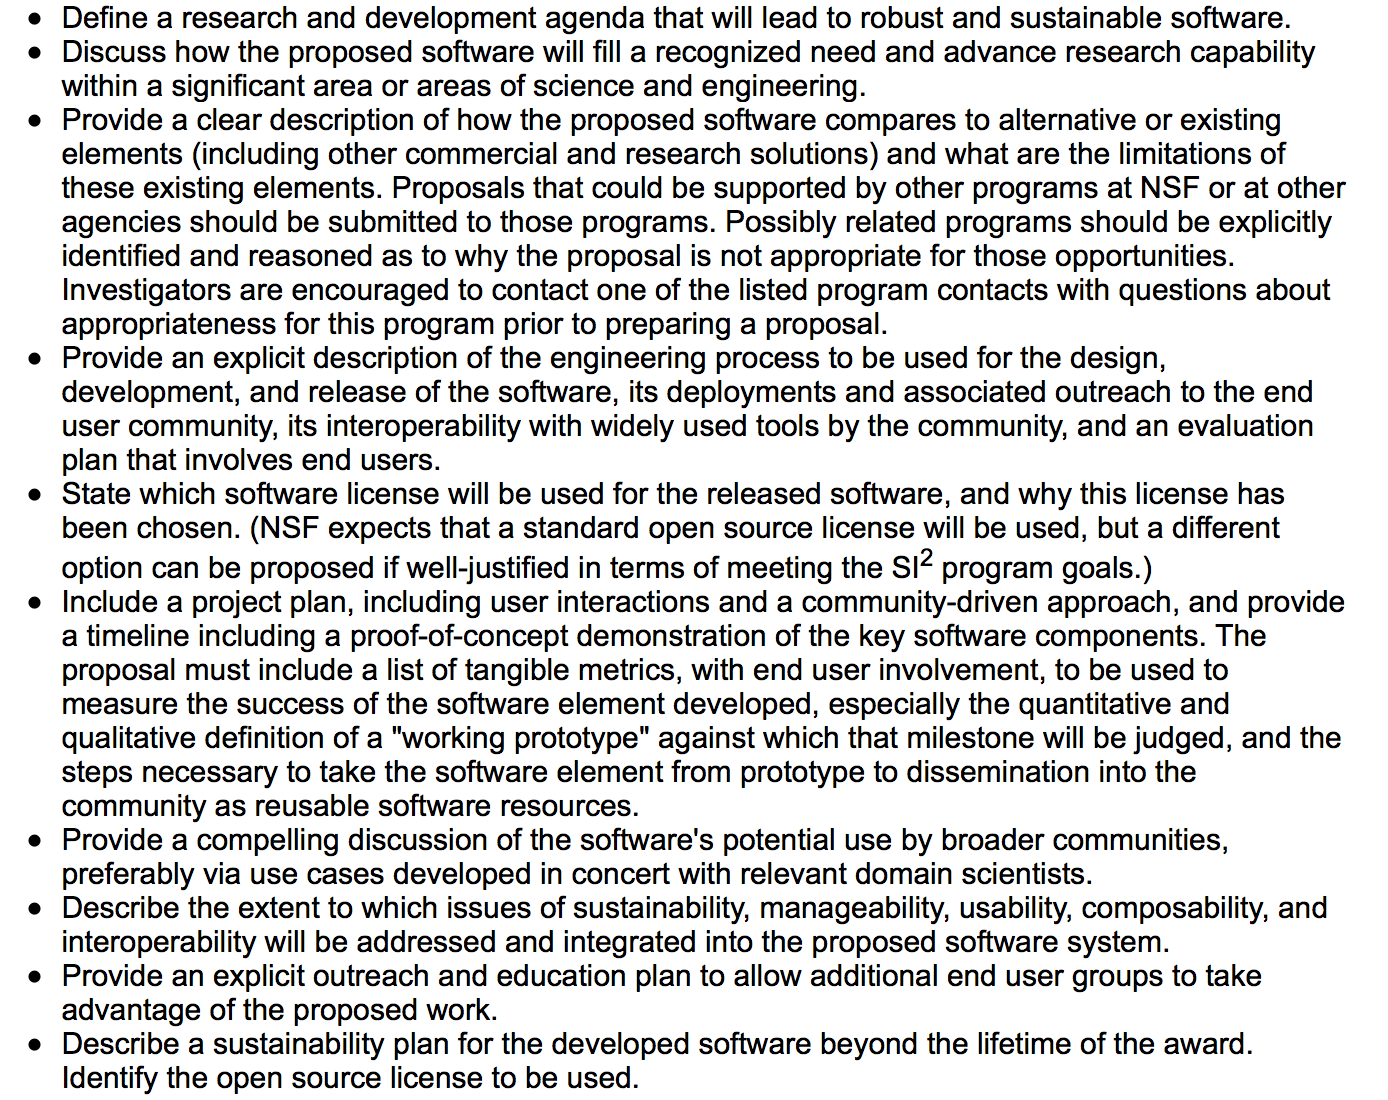
\includegraphics[width=0.9\textwidth]{images/nsf-si2-ssi-solicitation.png}
%%\caption{}
%%\label{fig:example2}
%\end{center}
%\end{figure}

\footnotesize{
A research and development agenda that leads to robust and sustainable software, that advances research capability for one or more areas of science 
\vskip 0.12in
Focus on the engineering process used for the design, development, and release of the software, its deployments and associated outreach to the end user community, its interoperability with widely used tools by the community, and an evaluation plan that involves end users.
\vskip 0.12in
Tangible metrics, with end user involvement, to be used to measure the success of the software developed, and the steps necessary to take the software elements from prototype to broader use
\vskip 0.12in
How can the software be used by broader communities? 
\vskip 0.12in
Issues of sustainability, manageability, usability, composability, and interoperability 
\vskip 0.12in
An outreach and education plan to allow additional end user groups to take advantage of our work.
\vskip 0.12in
How will the developed software be sustained beyond the lifetime of the project?
}

\end{frame}


